%-*-latex-*-

\begin{center}
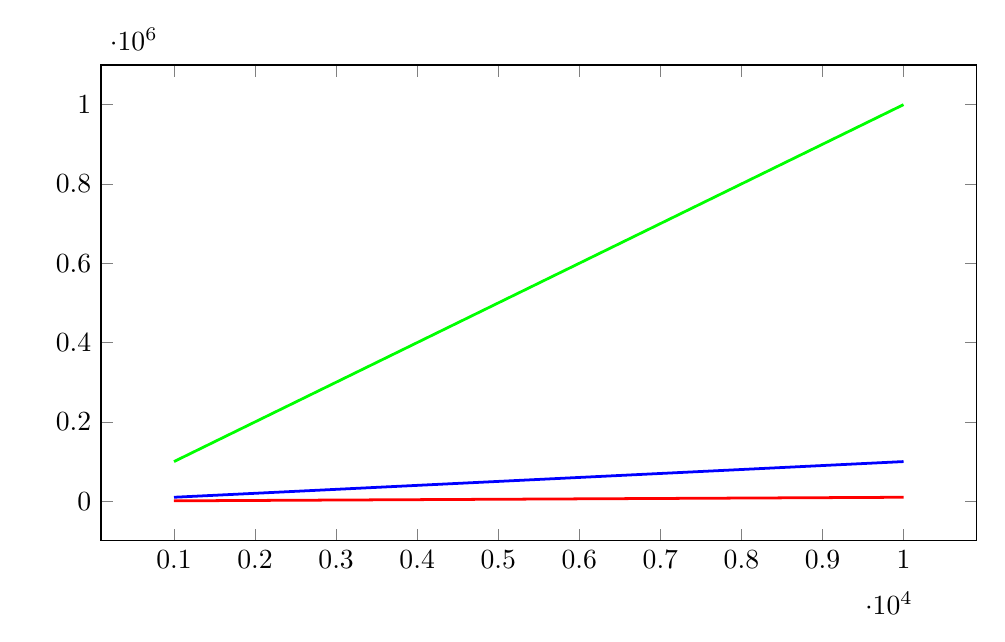
\begin{tikzpicture}[line width=1]
\begin{axis}[width=5in, height=3in,
             scatter/classes={a={mark=*,draw=black}},
             xlabel={\mbox{}},
             xlabel style={name=xlabel}, 
             ylabel={\mbox{}}, 
             legend style={
                at={(xlabel.south)},
                yshift=-1ex,
                anchor=north,
                legend cell align=left,
                },
        ]
]
\addplot[draw=red, line width=1] coordinates {(1000.0,1000.0)
(5500.0,5500.0)
(10000.0,10000.0)
(10000.0,10000.0)};\addplot[draw=blue, line width=1] coordinates {(1000.0,10000.0)
(5500.0,55000.0)
(10000.0,100000.0)
(10000.0,100000.0)};\addplot[draw=green, line width=1] coordinates {(1000.0,100000.0)
(5500.0,550000.0)
(10000.0,1000000.0)
(10000.0,1000000.0)};
\end{axis}\end{tikzpicture}\end{center}
